\documentclass[11pt]{article}
\usepackage[T1]{fontenc}
\usepackage[utf8]{inputenc}
\usepackage[sort]{natbib}
\usepackage{amsmath, amssymb}
\usepackage{fancyhdr}
\usepackage{dsfont}
\usepackage{graphicx}
\usepackage{float}
\usepackage{subfig}
\usepackage{pdfpages}

%\usepackage{fancyvrb}

%‎\usepackage{caption}‎
%‎\usepackage{color,xecolor}‎
%‎\usepackage[framed,numbered,autolinebreaks,useliterate]{mcode}‎
%\lstset{breakatwhitespace=false}
\usepackage[numbered, autolinebreaks, framed]{mcode}		% codice matlab
%\lstset{breaklines=true,breakatwhitespace=true,prebreak=\usebox{\lbreakdots}}
\usepackage{enumitem}						% elenco puntato
\renewcommand{\labelenumi}{\alph{enumi}.} 	% Make numbering in the enumerate environment by letter rather than number (e.g. section 6)	


%----- you must not change this -----------------
\oddsidemargin 0.2cm
\topmargin -1.0cm
\textheight 24.0cm
\textwidth 15.25cm
\parindent=0pt
\parskip 1ex
\renewcommand{\baselinestretch}{1.1}
\pagestyle{fancy}
\setlength{\headheight}{14pt}

%----------------------------------------------------



% enter your details here----------------------------------

\lhead{\normalsize \textrm{Roberto Costa}}
\chead{\normalsize Matricola: 1128285}
\rhead{Lab. 6}
\lfoot{\normalsize \textrm{Image and Video Anlysis}}
\cfoot{\thepage}
\rfoot{\normalsize Matricola: 1128285}
\setlength{\fboxrule}{4pt}\setlength{\fboxsep}{2ex}
\renewcommand{\headrulewidth}{0.4pt}
\renewcommand{\footrulewidth}{0.4pt}

\title{LABORATORY \#6: REPORT \\ A.A. 2015-2016} 
\author{Roberto \textsc{Costa}} % Author name
\date{\today}

\begin{document}
\maketitle
\begin{center}
\begin{tabular}{l r}
Subject: & Image and Video Analysis\\
Delivery date: & 31-05-2016 \\ 
Professor: & P. Zanuttigh \\
Student number: & 1128285
\end{tabular}
\end{center}


% If you wish to include an abstract, uncomment the lines below
%\begin{abstract}
% Abstract text
%\end{abstract}

\section{Motion detection}
The purpose of the lab is to develop an algorithm to detect the motion on some video.\\
The problem to estimate the motion on a video can be solved by estimating the motion between two adjacent frames of the video. The problem can be solved by estimating the SIFT feature between the two images and by finding the corresponding vector for each SIFT feature. The approach just descripted is computationally expensive and it is not used on some real time applications.\\
The algorithm is developed under the assumption of color constancy between two images, the assumption of small motion and the assumption of $I(x,y,t)$ differentiable.\\
The first assumptions can be formalized by the folowing equation
\begin{equation}
\label{eq:constancy}
I\left(x\left(t+\Delta t\right),y\left(t+\Delta t\right),t+\Delta t\right)
-I\left(x\left(t\right),x\left(t\right),t\right)=0
\end{equation}
By Taylor approximation of the first term of the sum, we can write
\begin{equation}
\label{eq:taylor}
I\left(x\left(t+\Delta t\right),y\left(t+\Delta t\right),t+\Delta t\right)\sim
I\left(x\left(t\right),y\left(t\right),t\right)
+\frac{\partial I}{\partial x} \frac{\partial x}{\partial t} \Delta t
+\frac{\partial I}{\partial y} \frac{\partial y}{\partial t} \Delta t
+\frac{\partial I}{\partial t} \frac{\partial t}{\partial t} \Delta t
\end{equation}
By combining eq. (\ref{eq:constancy}) and (\ref{eq:taylor}) we get
\begin{equation}
\label{eq:eq0}
\frac{\partial I}{\partial x } v_x + \frac{\partial I}{\partial y} v_y+ \frac{\partial I}{\partial t} = 0
\end{equation}
which can be written as
\begin{equation}
\label{eq:manyUnknown}
\left[ \Delta I (p_i)\right]^T
\begin{bmatrix}
v_x\\
v_y
\end{bmatrix} + I_t (p_i) = 0
\end{equation}
For each pixel, the eq. (\ref{eq:manyUnknown}) cannot be solved because te constraints are not enough with respect to the unknown variables.\\
This problem can be solved by imposing additional constraints, which pratically means to evaluate the equation for a window of pixel in the neighborhood.
\begin{equation}
\label{eq:eq1}
\begin{bmatrix}
I_x(p_1) & I_y(p_1)\\
I_x(p_2) & I_y(p_2)\\
\cdots & \cdots\\
I_x(p_{N^2}) & I_y(p_{N^2})\\
\end{bmatrix}
\begin{bmatrix}
u\\
v
\end{bmatrix}
= - 
\begin{bmatrix}
I_t(p_1)\\
I_t(p_2)\\
\cdots\\
I_t(p_{N^2})
\end{bmatrix}
\end{equation}
where a squared window of size $N$ is used.\\
The target to minimize the first term of eq. (\ref{eq:eq0}) can be achieved by minimizing the norm of it. By calling the first matrix of the first term of eq. (\ref{eq:eq1}) "$A$", the second matrix of the first term $d$ and the second term $b$, we can write $A d = b$. By pre-multiplicating both terms of eq. (\ref{eq:eq1}) by $A^T$ we get
\begin{equation}
A^T A d = -A^T b
\end{equation}
\begin{figure}[H]
	\centering
	{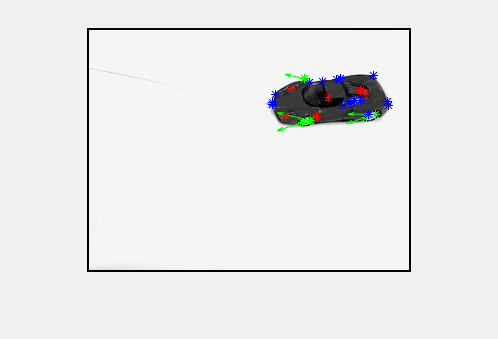
\includegraphics[width=12cm]{images/out_1_66_w2x2.png} }
    \caption{Output video 1, frame \# 66, window size: 2x2 pixels}
    \label{fig:out1_1}
\end{figure}

\begin{figure}[H]
	\centering
	{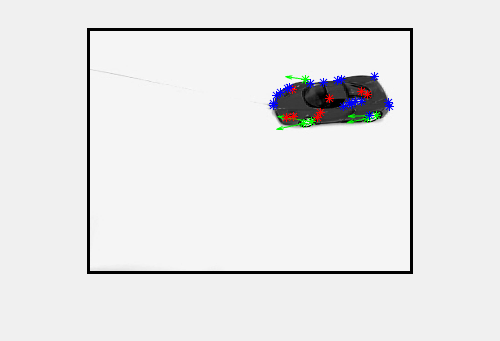
\includegraphics[width=12cm]{images/out_1_66_w3x3.png} }
    \caption{Output video 1, frame \# 66, window size: 3x3 pixels}
    \label{fig:out1_2}
\end{figure}

\begin{figure}[H]
	\centering
	{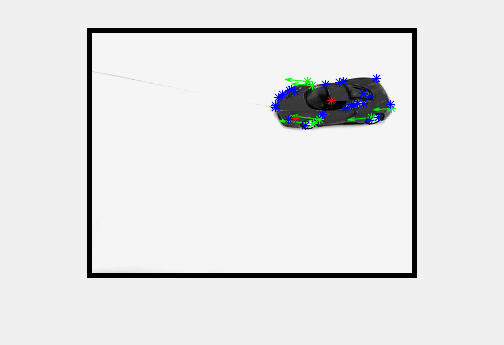
\includegraphics[width=12cm]{images/out_1_66_w5x5.png} }
    \caption{Output video 1, frame \# 66, window size: 5x5 pixels}
    \label{fig:out1_3}
\end{figure}

\begin{figure}[H]
	\centering
	{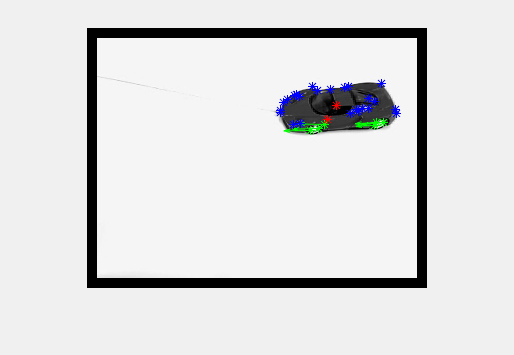
\includegraphics[width=12cm]{images/out_1_66_w10x10.png} }
    \caption{Output video 1, frame \# 66, window size: 10x10 pixels}
    \label{fig:out1_4}
\end{figure}

\begin{figure}[H]
	\centering
	{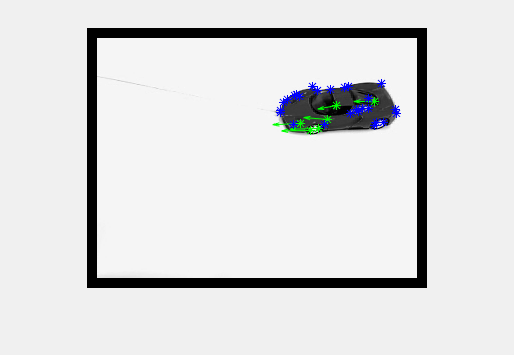
\includegraphics[width=12cm]{images/out_1_66_w10x10_2.png} }
    \caption{Output video 1, frame \# 66, window size: 10x10 pixels, different thresholds}
    \label{fig:out1_5}
\end{figure}

\begin{figure}[H]
	\centering
	{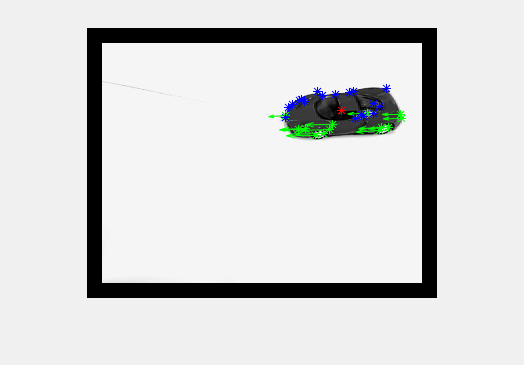
\includegraphics[width=12cm]{images/out_1_66_w15x15.png} }
    \caption{Output video 1, frame \# 66, window size: 15x15 pixels}
    \label{fig:out1_6}
\end{figure}

\begin{figure}[H]
	\centering
	{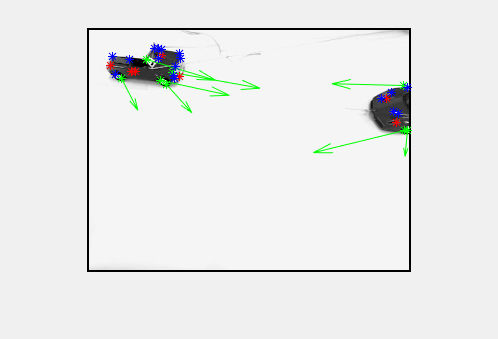
\includegraphics[width=12cm]{images/out_2.png} }
    \caption{Output video 2}
    \label{fig:out2}
\end{figure}


\end{document}
